\section{Análise de Resultados}

Foram realizadas 12 combinações de treinamento e teste: dois algoritmos de classificação (\textit{LinearSVC} e \textit{MultinomialNB}), treinamento com e sem validação cruzada e treinamento de três tipos de ato distintos (ADE, SC e PORT). As tabelas \ref{tab:resultados-ade}, \ref{tab:resultados-sc} e \ref{tab:resultados-port} apresentam os resultados para cada tipo de ato.

\begin{table}[h]
\caption{Resultados para os atos do tipo ADE}
\label{tab:resultados-ade}
	\begin{center}
	\begin{tabular}{lrrrr}
		\toprule
		{} &  Acurácia &  Precisão &  Revocacão &      F1-Score \\
		\midrule
		LinearSVC-1xR        &    0.9813 &    0.9764 &     0.9754 &  0.9759 \\
		MultinomialNB-1xR    &    0.9297 &    0.9282 &     0.9258 &  0.9259 \\
		LinearSVC-1xR-CV     &    0.9720 &    0.9630 &     0.9649 &  0.9636 \\
		MultinomialNB-1xR-CV &    0.9157 &    0.9083 &     0.9129 &  0.9090 \\
		\bottomrule
	\end{tabular}
	\end{center}		
\end{table}

\begin{table}[h]
\caption{Resultados para os atos do tipo SC}
\label{tab:resultados-sc}
	\begin{center}
	\begin{tabular}{lrrrr}
		\toprule
		{} &  Acuracia &  Precisão &  Revocação &      F1-Score \\
		\midrule
		LinearSVC-1xR        &    0.9906 &    0.9933 &     0.9872 &  0.9902 \\
		MultinomialNB-1xR    &    0.8291 &    0.9043 &     0.8088 &  0.8278 \\
		LinearSVC-1xR-CV     &    0.9780 &    0.9860 &     0.9619 &  0.9730 \\
		MultinomialNB-1xR-CV &    0.8129 &    0.8507 &     0.7950 &  0.7968 \\
		\bottomrule
	\end{tabular}
	\end{center}		
\end{table}

\begin{table}[h]
\caption{Resultados para os atos do tipo PORT}
\label{tab:resultados-port}
	\begin{center}
	\begin{tabular}{lrrrr}
		\toprule
		{} &  Acurácia &  Precisão &  Revocação &      F1-Score \\
		\midrule
		LinearSVC-1xR        &    0.8953 &    0.9075 &     0.8783 &  0.8914 \\
		MultinomialNB-1xR    &    0.7511 &    0.8370 &     0.6881 &  0.7212 \\
		LinearSVC-1xR-CV     &    0.8387 &    0.8538 &     0.8141 &  0.8285 \\
		MultinomialNB-1xR-CV &    0.6999 &    0.7850 &     0.6410 &  0.6619 \\
		\bottomrule
	\end{tabular}
	\end{center}		
\end{table}

Com base nos resultados encontrados, é possível concluir que os modelos treinados com o algoritmo \textit{LinearSVC} apresentaram melhor desempenho em todas métricas para todos os tipos de ato se comparados aos modelos treinados com o algoritmo \textit{MultinomialNB}. A diferença nos resultados dos treinamentos com e sem validação cruzada era esperada, visto que a validação cruzada estabelece um cenário de teste mais rigoroso, de forma evitar sobreajuste (\textit{overfitting}). Sendo assim, o melhor resultado, considerando as métricas utilizadas e o potencial de generalização do modelo, pode ser identificado como \textbf{LinearSVC-1xR-CV} nas referidas tabelas. 

Refinando a análise, se considerarmos somente o melhor resultado (\textit{LinearSVC} com validação cruzada), é possível constatar um resultado significativamente inferior para os atos do tipo PORT (com todas as métricas abaixo de 86\%) em comparação com os atos ADE e SC (que obtiveram valores acima de 96\% em todas as métricas). Para compreender melhor essa diferença, foram analisadas as matrizes de confusão referentes aos atos do tipo ADE e PORT.

A figura \ref{fig:matriz-confusao-ade} evidencia que a zona de maior confusão para os atos ADE está relacionada aos segmentos do tipo ``Não Identificado''. É possível perceber que os segmentos não identificados se confundiram com todos os outros tipos, gerando tanto falsos positivos quanto falsos negativos. Um resultado pior para a classificação de segmentos não identificados já era esperado, em virtude da natureza desse tipo de segmento, conforme discutido na seção \ref{sec:dist-atos-segmentos} da análise exploratória. Esse foi um problema que afetou não somente os atos do tipo ADE, mas também os atos SC e PORT. A situação dos segmentos não identificados indica a necessidade de abordagens adicionais que extrapolam o escopo da presente pesquisa, como a utilização de estratégias não supervisionadas para melhor entendimento da natureza dos dados desse tipo de segmento. Outra possibilidade é indicação de uma revisão manual dos segmentos não identificados para correção de possíveis omissões na classificação original realizada manualmente.

\begin{figure}[h]
	\caption{Matriz de confusão para atos do tipo ADE}
	\center
	\label{fig:matriz-confusao-ade}
	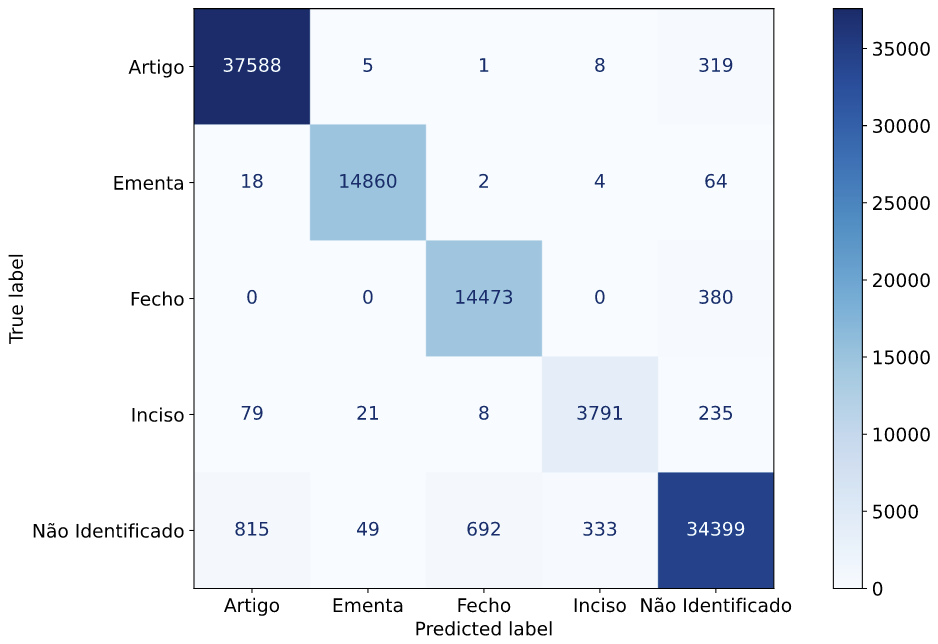
\includegraphics[scale=0.45]{resultados/matriz-confusao-ade.png}
	\fdp
\end{figure}

Especificamente no que tange os resultados obtidos com os atos do tipo PORT, a matriz de confusão (figura \ref{fig:matriz-confusao-port}) indica que, além do problema com os segmentos não identificados, houve confusão entre os segmentos dos tipos ``Alínea'', ``Inciso'' e ``Parágrafo''. Os atos PORT possuem uma representatividade maior dos tipos de segmento em questão em comparação com os atos ADE e SC. Além disso, esse é o tipo de ato com maior número de classes com 7 tipos de segmento, enquanto os atos ADE possuem 5 e os atos SC possuem 3.

\begin{figure}[h]
	\caption{Matriz de confusão para atos do tipo PORT}
	\center
	\label{fig:matriz-confusao-port}
	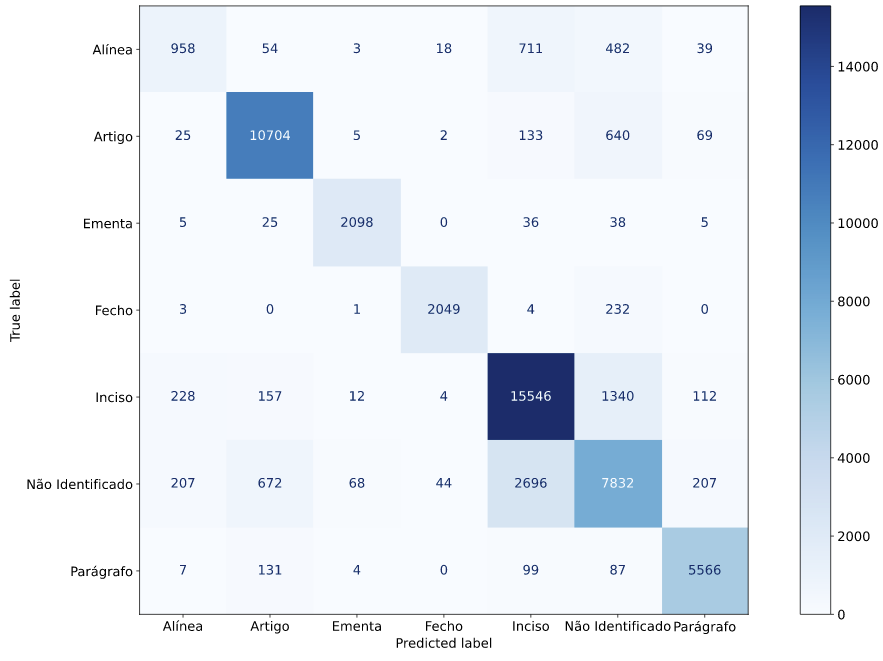
\includegraphics[scale=0.53]{resultados/matriz-confusao-port.png}
	\fdp
\end{figure}